\chapter{Modelado de los datos: ordenación de los usuarios}
\label{chap:ordenacion_de_usuarios}

\section{Principales hip\'otesis}
Una vez que ya tenemos una lista de usuarios cuyas publicaciones en Twitter
indican que podrían ser candidatos para las ofertas de trabajo, el siguiente
paso es ordenarlos por orden de relevancia. A continuación describimos brevemente
los dos criterios que usaremos para ordenarlos (el detalle de los algoritmos y 
procedimientos llevados a cabo en cada caso se hará en la secciones siguientes):
\begin{itemize}
\item Ordenación de tipo índice $h$. El índice h es un sistema propuesto por Jorge Hirsch, de la Universidad de California, para la medición de la calidad profesional de los científicos, en función de la cantidad de citas que han recibido sus artículos científicos\footnote{\url{https://en.wikipedia.org/wiki/H-index }}. Un científico tiene índice $h$ si ha publicado $h$ trabajos con al menos $h$ citas cada uno.  El índice se diseñó para medir eficazmente la calidad del investigador, a diferencia de sistemas de medición más sencillos que cuentan citas o publicaciones, donde se hace una distinción entre aquellos investigadores que tienen una gran influencia en el mundo científico de aquellos que simplemente publican muchos trabajos. En nuestro campo, lo que queremos es medir 
la relevancia de los candidatos, así que una métrica de este tipo aplicada a los tuits publicados
de la temática de interés (Big Data y ciencia de datos en nuestro caso), nos ayudará a determinarla.
Los detalles, en la sección \ref{subsect:indice_h}.

\item Ordenación en función del papel de cada usuario dentro de la red de usuarios
seleccionados (sección \ref{subsect:grafo}). Para ello, construiremos el grafo 
de los candidatos y sus relaciones, siendo estas relaciones dirigidas (A está relacionado
con B si A sigue a B).
\end{itemize}

Con estos dos métodos pensamos que quedará bastante bien representado el panorama
de candidatos a partir de la información extraída de Twitter. 
Todos los cálculos descritos en esta parte del proyecto están en el archivo
{\bf ordenacion\_usuarios.py} del repositorio de GitHub.

\section{Algoritmos}
En esta sección detallamos los algoritmos que hemos usado para cada sistema de
clasificación, aportando la justificación de las diversas elecciones que 
hemos llevado a cabo.
\subsection{Índice h}
\label{subsect:indice_h}
La particularización del índice $h$ a nuestro contexto podría ser 
del siguiente modo: un usuario de Twitter tendrá índice $h$ si $h$ de sus $N$ tuits
sobre un determinado tema, han sido retuiteados al menos $h$ veces.

Calcular el índice $h$ implica por tanto los siguientes pasos:
\begin{enumerate}
\item Explorar el timeline\footnote{\lq\lq Timeline\rq\rq es la palabra
que usan en Twitter para referirse a un flujo de publicaciones a lo largo del tiempo.
El timeline de un usuario es el flujo de las publicaciones de ese usuario.} 
de cada usuario. Para ello usaremos la función
{\tt user\_timeline} que ofrece el paquete de Python {\tt Tweepy}. 
\item Determinar, dentro de ese timeline, qué tuits son del tema que nos interesa
(Big Data o ciencia de datos) y descartar el resto.
\item De cada tuit publicado sobre el tema de interés, anotar su número de 
retuits y calcular el índice $h$. 
\end{enumerate}

La descarga del timeline de usuarios tienen varias limitaciones en el acceso a través 
del API de Twitter\footnote{\url{https://developer.twitter.com/en/docs/tweets/timelines/api-reference/get-statuses-user_timeline }}:
\begin{itemize} 
\item límite de $1500$ llamadas por cada ventana de $15$ minutos,
\item solo se permite acceder a los $3200$ más recientes tuits de cada usuario,
\item el número de tuits descargados en cada llamada al API solo puede ascender a $200$.
\end{itemize}
Para que el proceso de obtención de datos no se pare cuando alcanzamos el límite
de llamadas (da un error), la función de {\tt Tweepy} permite incluir el parámetro 
{\tt wait\_on\_rate\_limit = True} para gestionar ese error y esperar a reanudar
el proceso cuando sea posible.

La función del API de Twitter para obtener el timeline de los usuarios no tiene 
la opción de buscar tuits de forma temporal (por ejemplo, los de los tres
últimos meses). Hemos optado por evaluar el timeline respecto a los últimos
$200$ tuits publicados por parecernos un número lo suficientemente amplio para 
el objetivo de clasificar los usuarios, si bien se podría incluir en el código la
gestión de un número mayor de tuits en el timeline (aumentando el número de
llamadas al API).

Un aspecto importante a la hora de evaluar el impacto del usuario es distinguir 
entre sus publicaciones originales y los retuits. De los tuits que componen el 
timeline, vamos a extraer la siguiente información:
\begin{itemize}
\item el número de tuits descargados(que 
en principio serán $200$, pero podrían ser menos),
\item el número de tuits sobre el tema de interés, y por tanto el
porcentaje de tuits de interés sobre el total de tuits evaluados,
\item sobre los tuits de interés, el porcentaje de aquellos que son retuits,
\item el índice $h$ de los tuits originales. Para calcular el índice $h$ 
contaremos tanto las veces que se ha retuiteado el tuit como las que ha sido
citado.
\end{itemize}

Al intentar bajar el timeline de algunos usuarios se pueden
obtener diversos mensajes de error (por ejemplo, porque el usuario tenga
protegido tu timeline, porque el usuario haya dejado de existir, etc.)
de forma que el proceso puede fallar. El código debe contemplar ese
caso y permitir que la ejecución continue con el resto de usuarios:

\myfigure{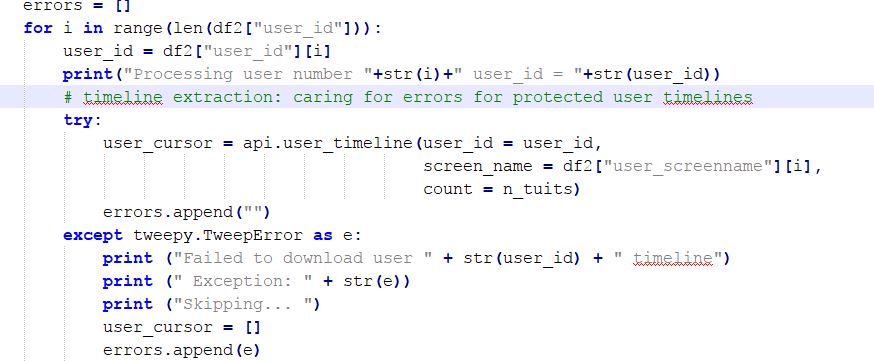
\includegraphics[width=0.6\textwidth]{error_not_authorized}%
\figcaption{Control de errores en la descarga de timelines.}
\label{fig:error_not_authorized} }


\subsection{Grafo relacional}
\label{subsect:grafo}
Nuestro objetivo en esta parte es explorar las relaciones entre los usuarios que 
hemos identificado como relevantes. De forma natural, como en cualquier red social,
se pueden definir multitud de estructuras de tipo grafo para describirlas. Nosotros
vamos a usar un grafo cuyos vértices serán los usuarios, y cuyas aristas serán
las relaciones entre ellos, de tipo dirigido: el usuario A está relacionado con el
usuario B si A sigue a B (y puede muy bien ocurrir que B no esté relacionado con A,
según esta definición). 

Para esta parte necesitaremos entonces descargar de Twitter la información
necesaria para construir el grafo de relaciones: los seguidores (\lq\lq followers\rq\rq)
y seguidos (\lq\lq friends\rq\rq) de cada uno de los usuarios identificados como
potenciales candidatos.

Y luego vamos a necesitar una librería para procesar el grafo y sacar las pertinentes 
conclusiones. A este respecto, tenemos varias opciones que considerar:
\begin{itemize}
\item {\tt Graph-tool}: los algoritmos están implementadas en una librería C++, 
lo que aporta mucha rapidez en la ejecución. Es 
buena procesando grafos grandes. La instalación en entornos Windows no
está soportada\footnote{\url{https://git.skewed.de/count0/graph-tool/wikis/installation-instructions 
}}.
\item {\tt NetworkX} es fácil de usar, para conjuntos de datos pequeños. Está bien
documentado.  Es compatible con Python 2.7, 3.4, 3.5 y 3.6.
\item {\tt  SNAP} (Stanford Network Analysis Platform): es un sistema para el análisis
y la manipulación de grandes redes. Está implementada en C++, con una interfaz en Python. 
Disponible para Python 2.7\footnote{\url{https://snap.stanford.edu/snappy/index.html }}.
\item {\tt igraph}: es una colección de herramientas para análisis de grafos,
con interfaces en R, Python y C/C++. Compatible con Python 2.6, 2.7 y 3.2.
\item {\tt APGL} (Another Python Graph Library): es una librería sencilla
para procesar grafos, disponible en principio para Python 2.7\footnote{\url{https://pythonhosted.org/apgl/ }}.
\end{itemize}

Vistas las opciones, nos hemos decidido por usar {\tt NetworkX}.

\section{Almacenamiento}